\section{Teórico}

  \definicion{Topic:} Time-dependent density-functional perturbation theory.

  \definicion{Speaker:} Iurii TIMROV (EPFL, Switzerland).

\subsection{Espectroscopia computacional: desde el estado basal hacia estados excitados}

  Todo lo visto hasta ahora permite describir el estado fundamental. Ahora queremos ver qué ocurre cuando excitamos los elecctrones para que pasen desde la banda de valencia hacia la banda de conducción.

  Para que los cálculos sean comparables con los experimentos, debemos incluir el dominio temporal en los mismos.

\subsection{Ecuación de Schrödinger dependiente del tiempo}

  Se sigue considerando la aproximación BO como en el caso estático. La ecuación de Schrödinger dependiente del tiempo establece la evolución de un sistema no relativista many-electrons interactuantes: no sólo se agrega la derivada temporal, sino que además se incorpora la variación temporal al término del potencial externo del Hamiltoniano del sistema.

  En vez de considerar las funciones de onda de $3N+1$ variables (3N posiciones más el tiempo), nuevamente consideramos la densdiad electrónica, la cual es una función de $4$ variables: $n (\vec{r}, t)$.

  Mientras que DFT es un mapeo uno-a-uno entre la densidad de carga y el potencial externo estático, mediante minimización de la energía total, una extensión directa de esta idea al dominio temporal no es posible debido a que la energía no es una cantidad conservada (no podemos establecer un principio variacional).

\subsection{Teoremas de Runge-Gross}

  El primer teorema establece que, dada una CI $\Psi (\vec{r},t_0) = \Psi_0 (\vec{r})$, para cualquier sistema de partículas interactuantes expuestas a un potencial externo dependiente del tiempo $V_{ext} (\vec{r}, t)$, existe un monomorfismo entre $V_{ext} (\vec{r}, t)$ y $n (\vec{r}, t)$, más allá de la solución trivial.

  Este teorema permite entones establecer una relación inyectiva entre el potencial externo y la densidad electrónica. Luego, tenemos nuevamente que todos los observables son funcionales de esta densidad de carga dependiente del tiempo: la diferencia es que necesitamos una CI.

  El segundo teorema establece que el funcional de acción $\mathcal{A}$ se vuelve estacionario una vez alcanzada la densidad electrónica exacta $n (\vec{r}, t)$ asociada al potencial externo $V_{ext} (\vec{r}, t)$ dada la CI $\Psi_0 (\vec{r})$.

  \Obs{Pensar en el formalismo de Lagrange.}

  Este segundo teorema establece que es posible resolver el problema dependiente del tiempo buscando el punto extremo de la acción en función de la densidad, pudiendo ser máximo o mínimo. El valor de la acción en sí mismo no ofrece información extra ya que se anula.

\subsection{Funcional de acción mecano-cuántico}

  El funcional de acción en el marco de DFT dependiente del tiempo (TDDFT) puede descomponerse de manera análoga al funcional de energía en DFT: un término cinético, uno de Hartree, uno XC y uno considerando el potencial externo.

  Para aproximar el funcional de acción, Gross y Kohn introdujeron un sistema auxiliar de partículas no interactuantes que satisfacen las ecuaciones KS dependientes del tiempo: ahora el potencial efectivo depende también del tiempo.

  \Obs{Es lo que hicieron KS a partir de HK en el caso independiente del tiempo.}

\subsection{Aproximación adiabática}

  En el caso dependiente del tiempo, el potencial XC depende del tiempo y de la densidad $n (\vec{r}, t)$ en todo momento pasado, dando lugar a una expresión mucho más compleja. La elección más usada es conocida como ALDA (Adiabatic LDA), la cual es obtenida a partir de evaluar el potecial LDA con la densidad $n (\vec{r}, t)$.
    $$V_{XC}^{ALDA} [n (\vec{r}, t)] = V_{XC}^{LDA} \left(n (\vec{r}, t)\right)$$

  Este presenta varias limitaciones: excitaciones dobles, excitaciones de transferencia de carga, etcétera.

\subsection{Regímenes en TDDFT}

  En TDDFT tenemos dos regímenes extremos:
    \begin{enumerate}
      \item \textbf{Respuesta lineal:} la perturbación es débil, permitiendo resolver el problema tanto en el dominio temporal como en el de frecuencias.
      \item \textbf{Respuesta no lineal:} la perturbación es fuerte, teniendo que resolver el problema en el dominio temporal necesariamente.
    \end{enumerate}

\subsection{TDDFPT: Linear-response TDDFT}

  Asumimos entonces que el potencial externo depende del tiempo, pero es débil. Esto nos lleva al régimen de respuesta lineal:
    $$V_{ext} (\vec{r}, t) = V_{ext}^0 (\vec{r}) + V_{ext}^{'} (\vec{r}, t)
    \Rightarrow
    n (\vec{r}, t) = n^0 (\vec{r}) + n^{'} (\vec{r}, t)$$

  La derivada primera de la densidad de carga viene dada por
    $$n^{'} (\vec{r}, t) = \int_{-\infty}^{\infty} \chi (\vec{r}, \vec{r}_0, t-t_0)) V_{ext}^{'} (\vec{r}_0, t_0) d \vec{r}_0 d t_0$$

  donde $\chi$ es la susceptibilidad del material.

\subsection{Cálculo de $\chi$ en TDDFPT}

  Existen al menos 4 métodos de linearizar y calcular la susceptibilidad para TDDFPT.

\subsubsection{Método de Dyson}

  La susceptibilidad es la variación de la densidad de carga respecto al potencial externo. Haciendo la regla de la cadena, se introduce el potencial KS con unas integrales. Éste a su vez es descripto como tres derivadas: de Hartree, de XC y de unas deltas de Dirac. Reescribe la variación del potencial de Hartree y del potencial XC (XC kernel). Se llega a que la susceptibilidad depende de sí mismma.

    \begin{figure}[H]
        \centering
        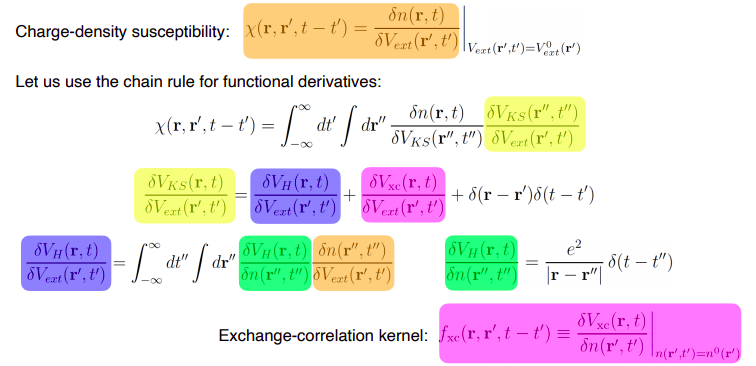
\includegraphics[scale = 0.6]{figs/D6/Dyson_1.png}
    \end{figure}

  Juntando todos los resultados se llega a una ecuación tipo Dyson, donde el término no integral se conoce como la polarizabilidad independiente de partículas $\chi^0$. Esta última función tiene picos cuando el denominador se anula: la energía del fotón entrante $\hbar\omega$ se iguala con la diferencia entre niveles $\epsilon_i - \epsilon_j$ (la singularidad se levanta con una cantidad infinitesimal Lorentziana).

    \begin{figure}[H]
        \centering
        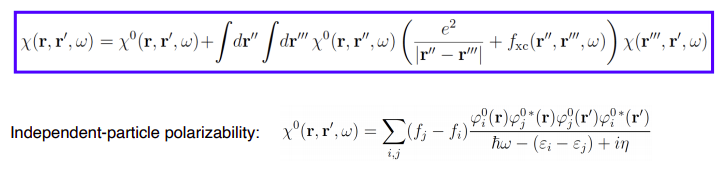
\includegraphics[scale = 0.6]{figs/D6/Dyson_2.png}
    \end{figure}

  Al pasar al espacio recíproco mediante FT pasamos de una ecuación integral a una ecuación matricial, con $q$ y $\omega$ fijos. A veces la ecuación se resuelve en la RPA (Random Phase Approxmation) donde se descarta la contribución XC.

  Finalmente, con DFT obtenemos la polarizabilidad independiente de partículas y luego con el método de Dyson obtenemos la susceptibilidad. Este método no está disponible en QE por todos estos problemas. Hay otras técnicas más avanzadas implementadas.

  Problemas:
    \begin{itemize}
      \item Sumar sobre estados vacíos para $\chi^0$. Estos son infinitos, hay que saber dónde cortar para la convergencia. Caro.
      \item Multiplicación e inversión de matrices muy grandes. Caro.
      \item Ambas matrices $\chi$ y $\chi^0$ deben ser resueltas para cada frecuencia de interés. Caro.
    \end{itemize}

\subsubsection{Método de Sternheimer}

  Escribimos el potencial externo como el término fundamental más la contribución dependiente del tiempo. Lo mismo para el potencial XC. Esto lleva a que el Hamiltoniano KS se pueda escribiir como una contribución fundamental más una contribución dependiente del tiempo. Luego, los estados KS son la suma del estado KS fundamental y una contribución TD, todo multiplicado por una fase temporal. A partir de esto reescribimos la ecuación KS en las ecuaciones de Sternheimer: una resonante y una antiresonante.

    \begin{figure}[H]
        \centering
        \subfigure[\empty]{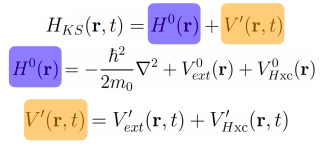
\includegraphics[scale = 0.6]{figs/D6/Stern_1.png}}
        \subfigure[\empty]{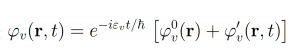
\includegraphics[scale = 0.6]{figs/D6/Stern_2.png}}
        \subfigure[\empty]{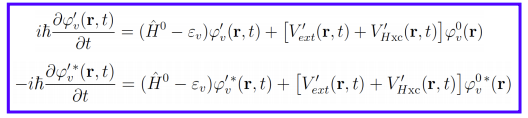
\includegraphics[scale = 0.6]{figs/D6/Stern_3.png}}
    \end{figure}

  Para resolverlas hacemos FT para ir del dominio temporal al de frecuencias.
    \begin{figure}[H]
        \centering
        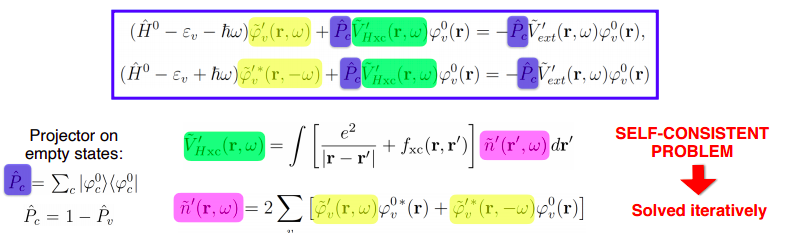
\includegraphics[scale = 0.6]{figs/D6/Stern_4.png}
    \end{figure}

  Vemos de vuelta que se muerde la cola: la densidad respuesta depende de las funciones de onda que son autoestados de las ecuaciones. Debemos recurrir a SCF. Lo bueno es que no necesitamos considerar estados vacíos ya que los proyectores sobre estados vacíos se pueden reescribir en términos de los proyectores sobre los estados ocupados. Sin embargo, seguimos necesitando resolver todo para cada frecuencia.

  \Obs{Si las frecuencias fueran nulas y los potenciales no dependieran de las frecuencias, las ecuaciones caen en el caso de DFPT para el cálculo de fonones.}

\subsubsection{Método de Liouville-Lanczos}

  Parte de la ecuación cuántica de Liouville (ecuación de von Neumann) que describe la evolución temporal del operador densidad de carga, la cual depende únicamente de las bandas de valencia. Usando teoría de respuesta lineal, se expande a primer orden la ecaución de Liouville.
    \begin{figure}[H]
        \centering
        \subfigure[\empty]{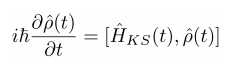
\includegraphics[scale = 0.6]{figs/D6/Liou_1.png}} \\
        \subfigure[\empty]{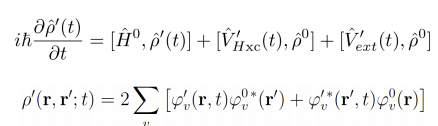
\includegraphics[scale = 0.6]{figs/D6/Liou_2.png}}
    \end{figure}


  Luego definimos el superoperador de Liouville y pasamos al dominio de frecuencias la ecuación linealizada. La solución formal a esta ecuación es mediante inversión matricial. Finalmente, la susceptibilidad del operador $A$ en función de la frecuencia será la traza del producto entre el observable y la densidad.
    \begin{figure}[H]
        \centering
        \subfigure[\empty]{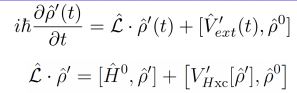
\includegraphics[scale = 0.6]{figs/D6/Liou_3.png}}
        \subfigure[\empty]{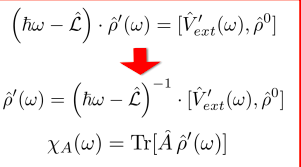
\includegraphics[scale = 0.6]{figs/D6/Liou_4.png}}
    \end{figure}

  En la práctica esto se resuelve recurriendo al método recursivo de Lanczos. Se define un standard batch representation: la semisuma y la semiresta de las fuciones de onda.
    \begin{figure}[H]
        \centering
        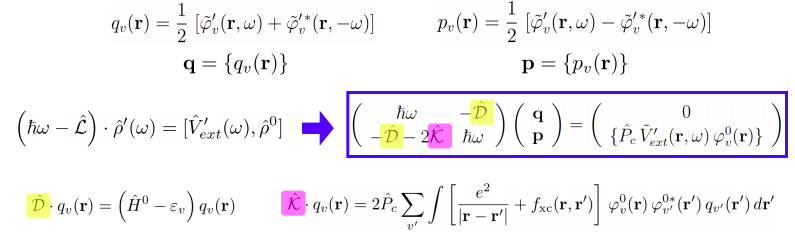
\includegraphics[scale = 0.6]{figs/D6/Liou_5.png}
    \end{figure}

  Luego se definen dos vectores de Lanczos bidimensionales y la cadena de recursión de Lanczos, junto a los coeficientes de Lanczos. Al resolverla se genera una matriz tridiagonal: es una matriz nula salvo en las diagonales $\pm 1$ respecto a la diagonal principal. Estos elementos tridiagonales corresponden a los coeficientes de Lanczos: los ceros de la diagonal principal son $\alpha$, mientras que los superiores son $\gamma$ y los inferiores son $\beta$. Finalmente, una vez que tenemos esta matriz construida podemos calcular la susceptibilidad buscada (sea hace PP y no es costoso).
    \begin{figure}[H]
        \centering
        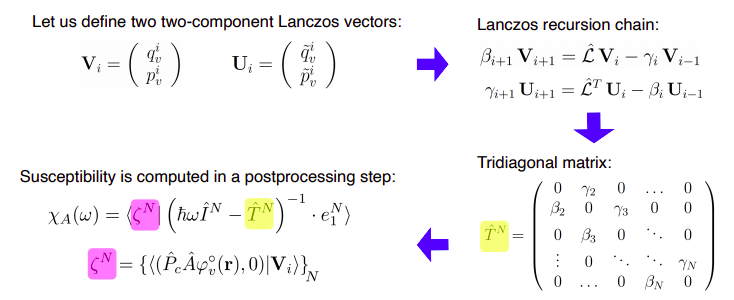
\includegraphics[scale = 0.6]{figs/D6/Liou_6.png}
    \end{figure}

  En resumen:
    \begin{itemize}
      \item No necesitamos considerar estados vacíos (misma razón que antes).
      \item La matriz tridiagonal se computa sólo una vez y es independiente de la frecuencia.
      \item El PP no es caro. Además la extrapolación de los coeficientes de Lanczos permite acelerar los cálculos.
    \end{itemize}

\subsubsection{Método de Casida-Davidson}

  Las ecuaciones de Casida parten de las ecuaciones de Sternheimer y anulan uno de sus miembros. Luego resuelve el problema de autovalores mediante un algoritmo de diagonalización tipo Davidson. Los autovalores corresponde a los polos de la susceptibilidad.
    \begin{figure}[H]
        \centering
        \subfigure[\empty]{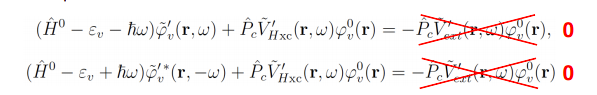
\includegraphics[scale = 0.6]{figs/D6/Casida_1.png}}
        \subfigure[\empty]{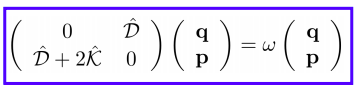
\includegraphics[scale = 0.6]{figs/D6/Casida_2.png}}
    \end{figure}

  \Obs{Mientras que el método de Sternheimer es útil para sólidos, el método de Casida es útil para sistemas moleculares, ya que no es práctico en sólidos debido a la alta densidad de estados que éstos presentan. El método de Liouville es útil tanto para sólidos como para moléculas.}

\subsection{Esepctroscopias}

  \begin{itemize}
    \item \textbf{Absorción óptica:} consideremos una perturbación externa asociada a un campo eléctrico homogéneo. Esta perturbación induce linealmente un dipolo. La conexión entre el dipolo generado y el campo aplicado es mediante el tensor de polarizabilidad dinámica (matriz 3x3).
      \begin{figure}[H]
          \centering
          \subfigure[\empty]{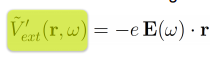
\includegraphics[scale = 0.6]{figs/D6/opt_1.png}}
          \subfigure[\empty]{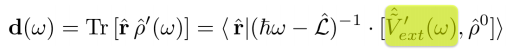
\includegraphics[scale = 0.6]{figs/D6/opt_2.png}}
          \subfigure[\empty]{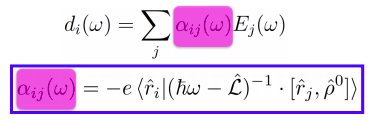
\includegraphics[scale = 0.6]{figs/D6/opt_3.png}}
      \end{figure}

    \item \textbf{Electron energy loss en sólidos:} ahora la perturbación no es un fotón, sino un electrón (una onda plana). Se mide el scaterring de los electrones.
      \begin{figure}[H]
          \centering
          \subfigure[\empty]{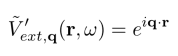
\includegraphics[scale = 0.6]{figs/D6/elec_1.png}}
          \subfigure[\empty]{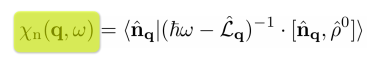
\includegraphics[scale = 0.6]{figs/D6/elec_2.png}}
          \subfigure[\empty]{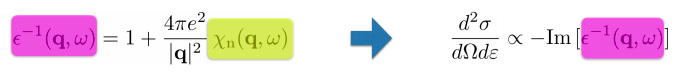
\includegraphics[scale = 0.6]{figs/D6/elec_3.png}}
      \end{figure}
    \item \textbf{Scattering inelástico de neutrones en sólidos:} ahora la perturbación es un neutrón, por lo que necesitamos considerar campos magnéticos.
      \begin{figure}[H]
          \centering
          \subfigure[\empty]{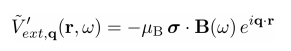
\includegraphics[scale = 0.6]{figs/D6/neu_1.png}}
          \subfigure[\empty]{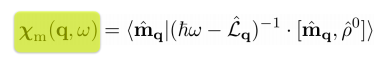
\includegraphics[scale = 0.6]{figs/D6/neu_2.png}}
          \subfigure[\empty]{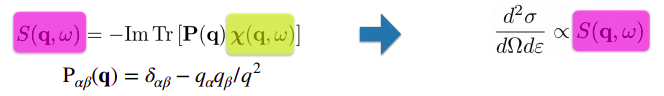
\includegraphics[scale = 0.6]{figs/D6/neu_3.png}}
      \end{figure}
  \end{itemize}

\subsection{Aspectos generales}

  \begin{itemize}
    \item TDDFPT permite el modelado de una gran variedad de espectroscopias a un costo computacional relativamente bajo cuando se usa la aproximación adiabática en comparación con teorías many-body.
    \item La aproximación adiabática da buenos resultados para muchas propiedades, pero sigue habiendo varias que no. En tal caso se debe agregar términos espaciales no locales y/o dependientes de la frecuencia en el término XC, lo cual dispara el costo computacional.
  \end{itemize}

\section{Q\&A}

  \definicion{As mentioned in the talk, for TDDFPT, we always need to give some initial condition. What i have understood from the exercises is that we are doing scf calcuation in order to provide this initial condition. Is it correct? If so, then we have to start with correct ground state calculations (after complete optimisation) otherwise we would end up with wrong spectra. Right? The 'precondition' flag (.true. by default)  in davidson.x input description is referring this condition?}

  Before any calculation (different by relax or scf), one should always have the correct ground state. So, this is always true. As far as the 'precondition' flag, it allows to speed up the convergence of the Davidson algorithm by introducing suitable procedures before the orthogonalization. It is well known that this provides very good results, reason why one should use its default value (.true.).

  \definicion{My other questions are also related to turbo\_davidson.x input: 1) according to input description, 'if\_dft\_spectrum = .true.' \& 'no\_hxc = .true.' both the options are there to consider IPA. Using anyone of them would work? or  if\_dft\_spectrum = .true. (as we used in example 01) is must?  2) How the value of 'num\_init' is decided? There it is written as 'num\_init' is usually twice of num\_eign. Is 'num\_eign' value is the number of bands we are calculating in scf step?}

  1) if\_dft\_spectrum = .true. is sufficient to perform a IPA calculation. Indeed, it allows to neglect the Hartree and exchange-correlation terms and, therefore, also their changes.

  2) In general, num\_init depends on the number of eigenvalues to calculate and, thus, on the system.

  3) num\_eign is the number of eigenvalues of the Casida's equations.

  \definicion{Does absorption spectroscopy calculations using these methods considers ground state to first excited state transition only?}

  No. Calculations provide all the transition peaks present in the user-specified frequency range with the user-specified interactions treatment.

  \definicion{hello, in many cases in Hands-on, we performed the postprocessing, we just calculate SCF and I assume that we have to perform the relax optimization before? am I right?}

  Yes, one has to optimize the structure before and then compute the spectrum. But in this hands-on, we skip this step in the interest of time

\section{Hands-on}

  \definicion{Topic:} TDDFPT.

  \definicion{Speaker:}	Iurii TIMROV (EPFL, Switzerland), Oscar BASEGGIO (SISSA, Italy).

\subsection{Espectro de absorción de benceno: método de Casida-Davidson}

  El ejecutable turbo\_davidson.x permite calcular el espectro de absorción de moléculas utilizando TDDFPT. Las interacciones electrónicas, tante de Hartree como XC, son tenidas en cuenta o despreciadas según $if\_dft\_spectrum$ (.true. es para IPA).

  Vamos a partir desde IPA (Independent Particle Approxmation) hacia electrones interactuantes. En el contexto de la IPA se tiene una suma de excitaciones independientes desde estados ocupados hacia estados vacíos.

  Como siempre arrancamos calculando el estado fundamental, pero ahora debemos aclarar $nbnd$ para pedirle explícitamente al código que calcule estados vacíos. Luego calculamos la respuesta lineal en IPA.
    \begin{verbatim}
      turbo_davidson.x < turbo_davidson.benzene.in > turbo_davidson.benzene.out
    \end{verbatim}

  Finalmente calculamos el espectro.
    \begin{verbatim}
      turbo_spectrum.x < turbo_spectrum.benzene.in > turbo_spectrum.benzene.out
    \end{verbatim}

  La resonancia más intensa corresponde a la primera excitación (diferencia entre LUMO y HOMO). La resonancia en torno a 8 eV es la siguiente excitación de mayor energía.
    \begin{figure}[H]
        \centering
        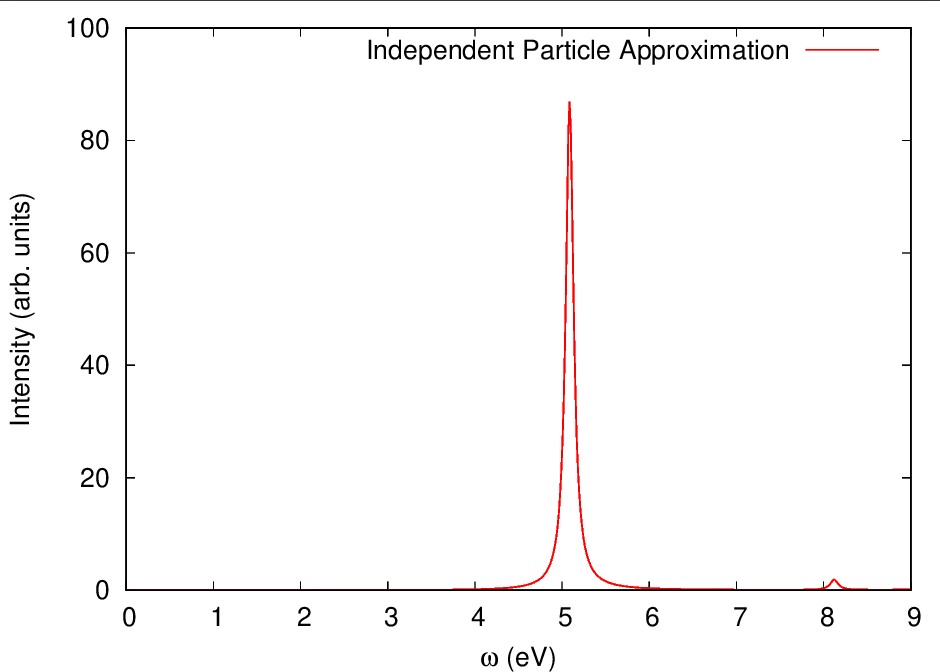
\includegraphics[scale = 0.6]{figs/D6/Benceno_IPA.png}
    \end{figure}

  Ahora vamos a prender las interacciones electrónicas. Para ello hay que modificar los inputs:
    \begin{itemize}
      \item En $turbo\_davidson.benzene.in$ poner
        \begin{itemize}
          \item if\_dft\_spectrum = .false.
          \item num\_eign = 15
          \item num\_init = 30
          \item num\_basis\_max = 90
          \item start = 0.0
          \item finish = 1.0
          \item step = 0.001
          \item broadening = 0.004
        \end{itemize}
      \item En $turbo\_spectrum.benzene.in$ poner $eign\_file = 'Benzene.eigen'$
      \item En $plot\_spectrum.gp$ cambiar la última línea por
        \begin{verbatim}
          "Benzene.plot.dat" u ($1)*13.6:($3) w l lw 2 lt rgb "blue" title 'with interactions', \
         "reference/no_interaction/Benzene.plot.dat" u ($1)*13.6:($3) w l lw 2 lt rgb "red" title 'no interactions'
        \end{verbatim}
    \end{itemize}

  Luego repetir los mismos pasos que antes. Vemos que el cálculo de respuesta lineal tarda mucho más que en IPA. La resonancia se corre hacia valores más altos ya que las interacciones aumentan el gap.
  \begin{figure}[H]
      \centering
      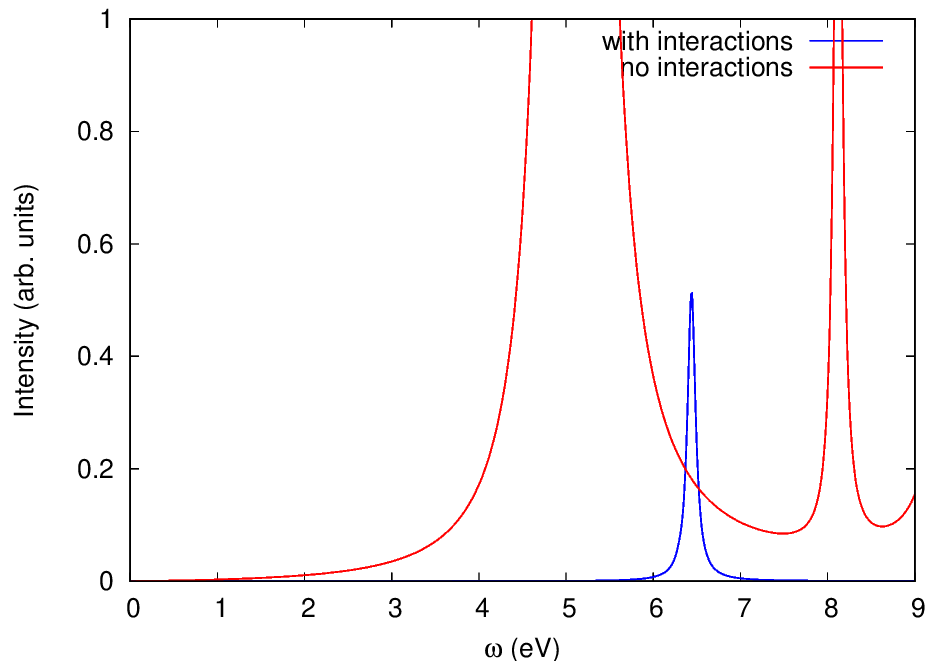
\includegraphics[scale = 0.6]{figs/D6/Benceno_inter.png}
  \end{figure}

\subsection{Espectro de absorción de benceno: método de Lanczos}

  Espectro total a bajo costo para electrones interactuantes.

  Esoectro: se pueden poner menos de la cantida total de iteraciones hechas, pero no más.

  A mayor cantidad de iteraciones va cambiando la ubicación de los picos. También cambian sus intensidades. Esto habla de que el espectro no está convergedio correctamente: hay que hacer más iteraciones o hacer un truco.

  Para el truco ver qué le pasa el beta de Lancszos: una extrapolación que aumenta el número de coeficientes sin calcularlos.















\subsection{Example 3}

  Los dos primeros estudiaban una molécula. Ahora vamos a estudiar un sólido.

  El calculator le dice si usar Lancszos o Sternheimer.

  q1, q2 y q3: componentes de la transferencia de momento.

  [me fui un buen tiempo]

  Siempre conviene hacer extrapolación porque ahorra una banda de tiempo.

  La definición del plasmon dice que el pico (de la imaginaria) ocurre en torno a la raíz de la parte real con pendiente positiva. Cuando la pendiente es negativa hay picos en le epsilon imaginaria.

\subsection{Example 4}

  Ejemplo más complejo de toda la escuela. Dos métodos bien distintos dan lugar a exactamente el mismo espectro.

  No tenemos las iteraciones (específicas de Lanczos), pero mantenemos las coordendasd del vector q. Hay otras palabras claves.

  Tarda unas 2 horas ya que no está del todo optimizado el código todavía.

  Dan igual espectro, pero el Lanczos le pasa el trapo en velocidad al Sternheimer. Aparece discreto porque hace un cálculo por frecuencia. Para tener un espectro más denso: más caro que eia.

  Obviamente que la convergencia de la k mesh hacerla con Lanczos. AL principio no es smooth pero a medida que avanza se suaviza.

  Dispersión plasmónica: el espectro va cambiando según el valor de la transferencia de momento. La dispersión plasmónica es la parábola que se forma al tomar las intensidades de los picos.
